\chapter{Analysen}\label{ch:method}

\section {Voruntersuchungen}
Wie in Abschnitt 2.3 bereits erwähnt, liegt eine hohe Usability genau dann vor wenn eine System von der für es bestimmten Zielgruppe effizient verwendet werden kann.\cite{Richter.2016}
Um dies zu gewährleisten ist es vorab nötig diese Zielgruppe zu kennen, zu analysieren und eventuelle Schwierigkeiten in der Benutzung des Systems aufzudecken.
Das Erkennen dieser Schwierigkeiten muss, aus Gründen die ebenfalls in Abschnitt 2.3 erläutert wurden, immer in Relation zu der aktuell ausgeführten Aufgabe geschehen, weshalb im Folgenden zuerst die Ausgangssituation beschrieben wird in der die Analysen durchgeführt wurden.
Anschließend folgt noch ein Überblick über die Analysemethoden, bevor abschließend die Ergebnisse dargestellt werden.

\subsection{Ausgangssituation}
Im ersten Schritt des Human-centered design process, zu sehen in \cref{fig:HCD} des vorherigen Kapitels, gilt es den Benutzungskontext zu verstehen.
Aus all den möglichen Aufgaben, die der User Requirements Engineer in diesem Schritt des Prozesses bearbeiten soll, wird in dieser Arbeit auf die Nutzergruppe, deren tägliche Aufgaben und die Arbeitsumgebung eingegangen.

\paragraph{Arbeitsumgebung}
Das Arbeitsumfeld bildet das in Abschnitt 2.8 bereits erwähnte EB Guide 6.
Es ist hierbei Situationsabhängig ob die Modellierer mit dem Speech Anteil von EB Guide arbeiten oder nicht, für diese Arbeit werden die Interaktionen mit dem Speech Teil ignoriert und sich nur auf die Usability von EB Guide Studio konzentriert.
Auch auf beide Target Frameworks wird im Folgenden nicht mehr weiter eingegangen, da die Nutzerinteraktion mit EB Guide über die Schnittstelle EB Guide Studio stattfindet.

\paragraph{Nutzergruppe}
Die Zielgruppe für die Analysen im Rahmen dieser Arbeit deckt sich logischerweise mit der Nutzergruppe von EB Guide.
Im Rahmen dieser Arbeit wurden nur Personen beobachtet und analysiert die bei Elektrobit beschäftigt sind.
Diese arbeiten teilweise bereits sehr routiniert und auch täglich mit der Software, andere benötigen diese nur sporadisch in ihrer täglichen Arbeit.
Es werden also Experten und gelegentliche Nutzer in dieser Arbeit untersucht, neue Nutzer werden nicht beachtet.
Wie in Abschnitt 2.3 nachvollziehbar ergeben sich hieraus theoretisch die Möglichkeiten das System auf Effizienz, Wiedererkennungswert, Fehler und Zufriedenheit zu testen, welche jedoch im Folgenden noch eingegrenzt werden.

\paragraph{Arbeitsaufgaben}
Der Großteil der Modellierer arbeitet in laufenden Projekten von Elektrobit und modelliert dort mithilfe von EB Guide 6 Human Machine Interfaces für die Automobilbranche.
Ein anderer Teil der Zielgruppe arbeiten an Kundendemonstrationen mit derern Hilfe dargestellt wird was mit der aktuellen Version von EB Guide 6 modelliert werden kann.
Beide Gruppen setzten bei ihrer Arbeit Spezifikationen um die nach den Wünschen des Kunden direkt von diesem oder von Designfirmen erstellt werden.
Diese Spezifikationen bestehen meist aus einem schriftlichen Teil der die Logik beschreibt nach der das Interface arbeiten muss, sowie aus einem grafischen Teil der die Anordnung von Icons und Texten zeigt.


\subsection{Vorgehensweise}
Nachdem nun der Benutzungskontext analysiert und verstanden wurde, gilt es im zweiten Schritt des Prozesses die Benutzeranforderungen zu spezifizieren.
Diese Benutzeranforderungen beinhalten die Definition identifizierter Bedürfnisse der Nutzer, sind testbar, eindeutig und konsistent.
Zu unterscheiden sind qualitative und quantitative Benutzeranforderungen, wobei beide eine Basis für das Design des interaktiven Systems bieten und durch Evaluierung des Systems verifiziert werden können.
Qualitative Anforderungen beziehen sich auf die Art und Weise wie das System genutzt wird um das Ziel zu erreichen, quantitative Anforderungen hingegen setzen messbare Ziele für die Usability und User Experience.\cite{.f}

Um repräsentative Benutzeranforderungen zu erhalten ist es notwendig, das die Bedürfnisse der Nutzer, aus denen die Anforderungen gebildet werden, tatsächlich auch den Bedürfnissen der Zielgruppe entsprechen.
Diese Bedürfnisse erhält man beispielsweise durch Interviews oder Beobachtungen innerhalb der Zielgruppe.
Diese Vorgehensweisen wird im Rahmen dieser Arbeit kombiniert angewendet.
Die Nutzer werden bei ihrer täglichen Arbeit beobachtet, werden währenddessen aufgefordert ihre aktuellen Arbeitsschritte zu erklären wodurch sie bei Bedarf auch automatisch Kritik am Interface äußern können.
Zusätzlich können durch den Beobachter begleitend Fragen gestellt werden.

\subsection{Ergebnisse}

Bei der Durchführung der Beobachtungen fallen einige Dinge auf die die Modellierer bei der Durchführung ihrer Arbeit behindern oder erheblich verlangsamen.
Teilweise fällt den Nutzern das selbst auf und sie weisen den Beobachter darauf hin, teilweise haben sie sich bereits so an die Arbeitsschritte gewöhnt das die Behinderung nur einem Außenstehenden auffällt, den Nutzern selbst jedoch kaum noch.

Im Folgenden werden zuerst Beobachtungen allgemein erläutert, bevor die Bedürfnisse der Nutzer formuliert werden, damit es abschließend möglich ist die Benutzeranforderungen zu definieren.

\paragraph{Image List}
Bei einer Image List handelt sich um ein Datapool Item. 
Datapool items sind Modelelemente die benutzt werden können um Daten von der Applikation an das Interface zu senden, oder umgekehrt.
Ebenfalls können damit Daten gespeichert werden die entweder nur von Seiten des Interfaces genutzt werden, oder nur von der Applikationsseite.\cite{studio_guide}
in \cref{fig:ImageList} kann das befüllen eines solchen Datapool items am Beispiel einer Image List nachvollzogen werden.
In Abbildung b) initialisiert der Nutzer das Befüllen der Liste durch einen Klick auf den "Stift" Button, wodurch sich das Pop Up in Abbildung c) öffnet.
Die hier zu sehenden Platzhalter für Index und Value müssen einzeln durch einen Klick auf den "Add.." Button hinzugefügt werden, und danach einzeln, wie in Abbildung d) zu sehen, mit dem gewünschten Image befüllt werden.
Für die minimale Auswahl in dem hier zu sehenden Beispiel ist der Aufwand noch erträglich, es ist jedoch zu bedenken das in tatsächlichen Projekten Image Lists mit mindestens 100 Images erstellt werden.
Das bedeutet für den Nutzer mehrere Stunden Arbeit, die keinen wirklich Mehrwehrt liefern und den Joy of Use deutlich mindern.
\begin{figure}%
  \centering
  \subfloat[][]{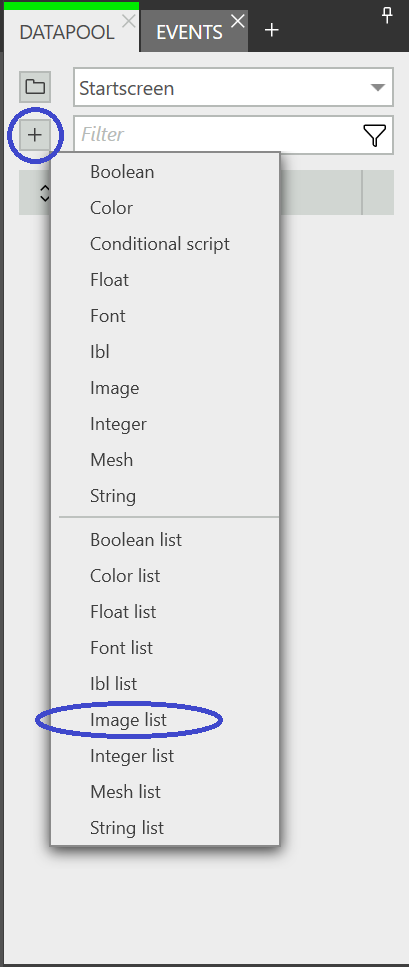
\includegraphics[width=0.3\linewidth]{figures/ImageList_01.PNG}}%
  \qquad
  \subfloat[][]{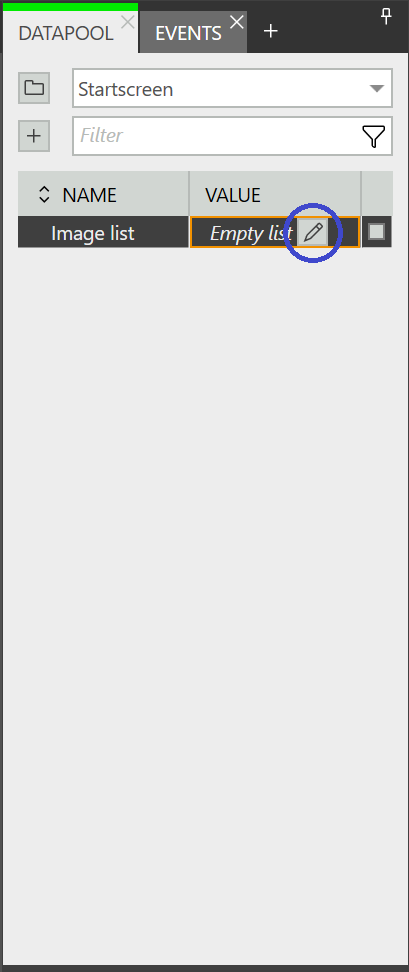
\includegraphics[width=0.3\linewidth]{figures/ImageList_02.PNG}}%
 \qquad
  \subfloat[][]{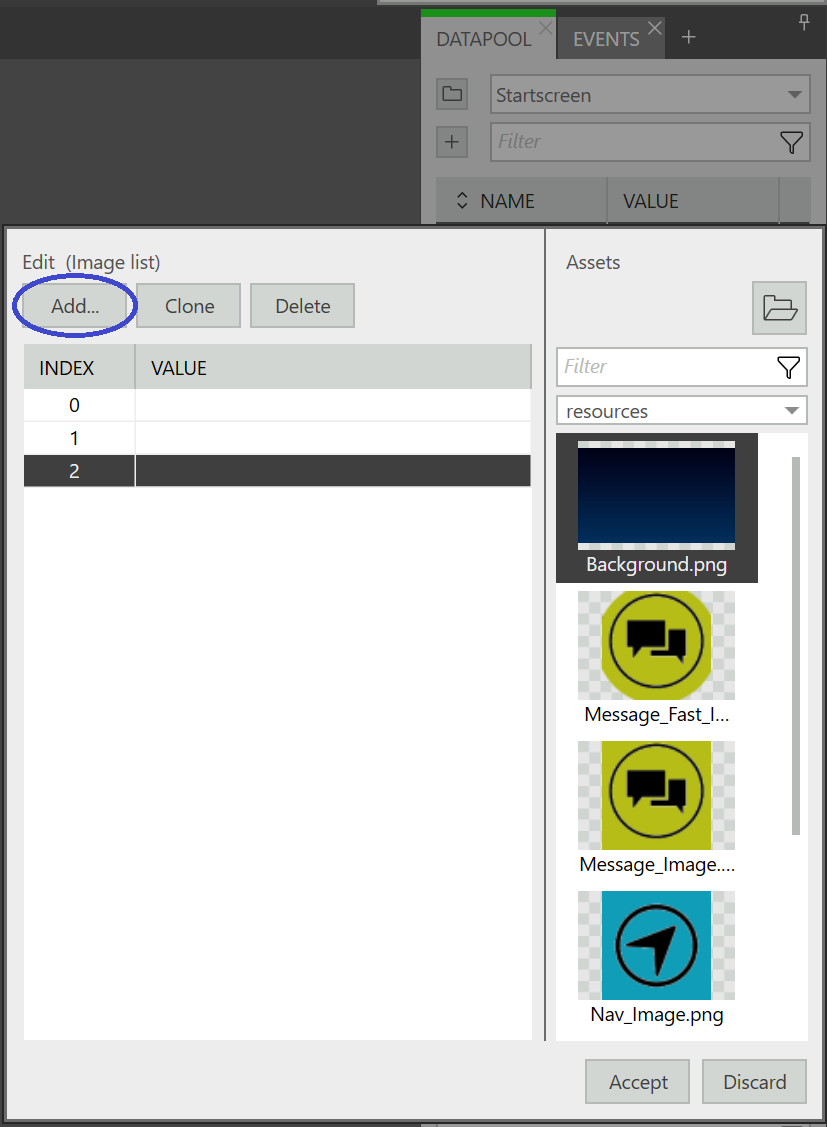
\includegraphics[width=0.4\linewidth]{figures/ImageList_04.PNG}}%
 \qquad
  \subfloat[][]{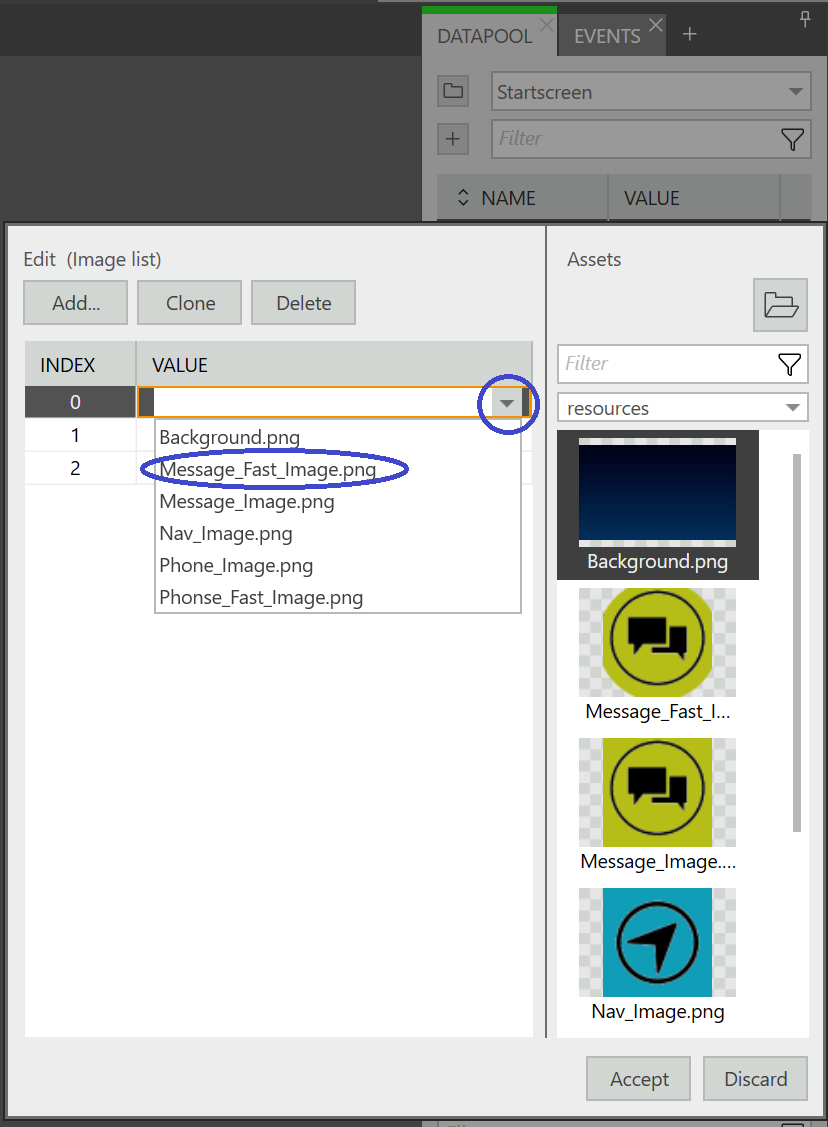
\includegraphics[width=0.4\linewidth]{figures/ImageList_05.PNG}}%
  \caption{Usability - Schwäche Image List}%
  \label{fig:ImageList}
\end{figure}

\paragraph{Resultierende Benutzeranforderung}
Nutzer, die eine Datapool Liste anlegen, müssen die Möglichkeit haben mehrere Images gleichzeitig zu dieser Liste hinzuzufügen.


\paragraph{Navigation}
Wird ein neues Element in der View hinzugefügt wird der WidgetTree in der Navigation, in \cref{fig:Navigation} zu sehen, nicht automatisch ausgeklappt.
Durch Beobachtung kann festgestellt werden das die Nutzer, nachdem sie ein neues Element eingefügt haben dieses sofort umbenennen. 
Für diesen Vorgang müssen sie das Element im WidgetTree erst gesucht werden, was in einigen Fällen sehr viele Klicks, und damit auch Zeit fordert.
Sollte der Nutzer in \cref{fig:Navigation} beispielsweise gerade das NavImage eingefügt haben, müssen erst vier Ebenen ausgeklappt werden bevor eine Umbenennung möglich ist.

\begin{figure}%
  \centering
  \subfloat[][]{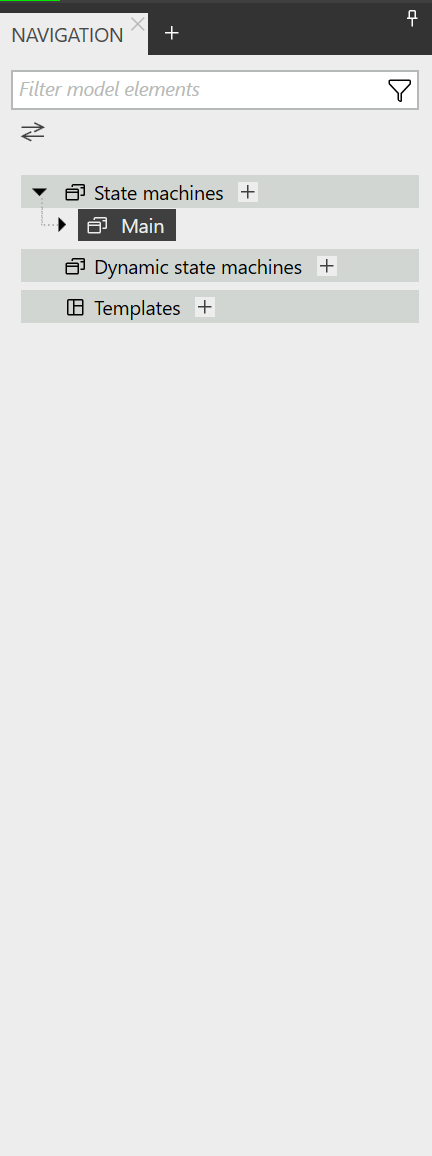
\includegraphics[width=0.4\linewidth]{figures/Navigation.png}}%
  \qquad
  \subfloat[][]{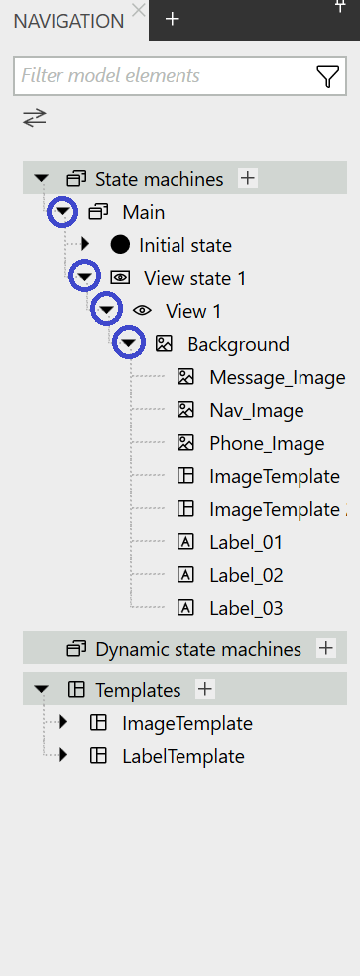
\includegraphics[width=0.4\linewidth]{figures/Navigation_01.png}}%
  \caption{Usability - Schwäche Navigationt}%
  \label{fig:Navigation}
\end{figure}

\paragraph{Resultierende Benutzeranforderung}
Nutzer, die ein neues Element zu ihrer View hinzufügen, müssen die Position dieses Items sofort im WidgetTree nachvollziehen können.

\paragraph{Template Properties}
Ein Widget Template ermöglicht die Definition eines individuellen Widgets, welches beliebig oft in einem EB Guide Model benutzt werden kann.
Es besteht die Möglichkeit Templates zu erstellen die auf bereits existierenden Widgets aufbauen, oder von einem anderen Template abgeleitet sind.
Nach der Erstellung kann das Template nach den eigenen Wünschen und Bedürfnissen angepasst werden, beispielsweise durch das hinzufügen von Properties.

Ein Widget Template besitzt außerdem ein Template Interface, welches jene Poperties beinhaltet des Templates beinhaltet welche für jeder Instanz des Templates sichtbar und veränderbar sein sollen.
Jede Instanz eines Templates erbst also die Properties des Template Interfaces, welche Template Properties genannt werden.\cite{studio_guide}

In \cref{fig:TemplateProperties} ist zu sehen wie die Funktion puplish to template interface ausgeführt wird.
Hierfür ist zuerst ein Rechtsklick auf das Viereck hinter dem gewünschten Propertie nötig, bevor noch auf Add to template interface geklickt werden muss.

Während der Beobachtung wird deutlich, das vor allem der Rechtsklick den Arbeitsablauf sehr beeinflusst, da dieser in EB Guide nicht häufig verwendet wird. 
Zum Gropßteil wird mit dem normalen Linksklick gearbeitet, weshalb das auch für diesen Fall wünschenswert wäre
In Teil b) von \cref{fig:TemplateProperties} sieht man, das das verlinkte Properties nun einen blauen statt einem weißen Kreis aufweist.
Alle anderen Optionen die durch den Rechtsklick geboten werden spiegeln sich Nach Anwendung farblich im Quadrat wieder und lassen den Kreis unberührt.
Es wäre also denkbar die Funktion puplish to template interface einfach durch einen Linksklick auf den Kreis zu aktivieren.

\begin{figure}%
  \centering
  \subfloat[][]{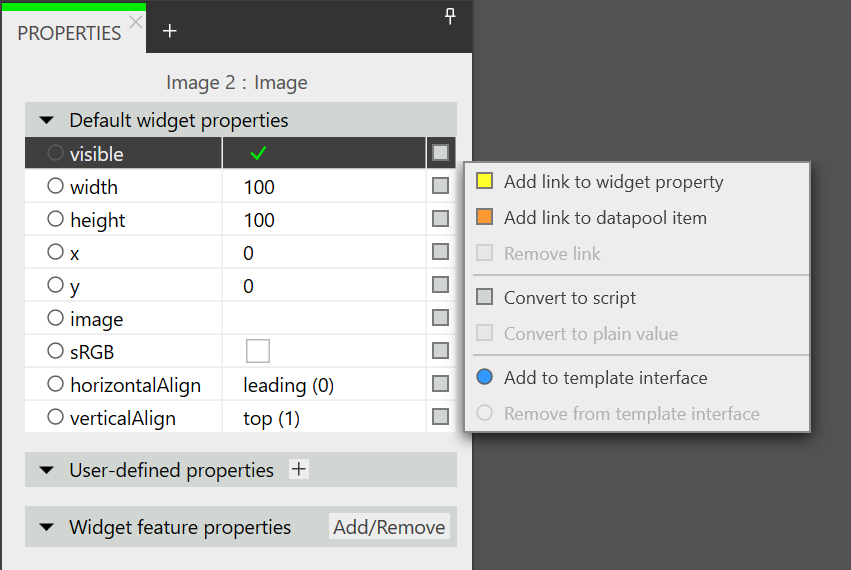
\includegraphics[width=0.4\linewidth]{figures/TemplateProperties.png}}%
  \qquad
  \subfloat[][]{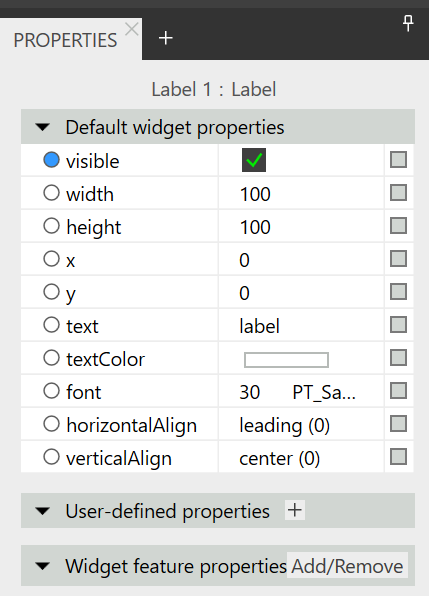
\includegraphics[width=0.4\linewidth]{figures/TemplateProperties_01.png}}%
  \caption{Usability - Schwäche Template Properties}%
  \label{fig:TemplateProperties}
\end{figure}


\paragraph{Resultierende Benutzeranforderung}
Nutzer, die für ein Propertie dir Funktion publish to template interface ausführen möchten,müssen dies auf eine intuitive und direkte Art und Weise tun können.

\paragraph{Widget Feature Properties}

Neben den Default Widget Properties  wie Breite und Höhe die jede Widgetinstanz besitzt, existieren noch die so genannten Widget Feature Properties.
Diese Features fügen mehr anpassbare Funktionen für das Aussehen und das Verhalten der Widgets bereit.
Wie in \cref{fig:WidgetFeatureProperty} zu sehen sind die Features in Kategorien unterteilt, die grafisch in Form eines Dropdownmenüs dargestellt sind.

Bei der Beobachtung der Nutzer fällt auf das viele Nutzer genau wissen welches Feature sie hinzufügen wollen, jedoch häufig die zugehörige Kategorie nicht präsent haben.
Dies führt dazu das jedes Dropdownmenü aufklappt wird, bis das gewünschte Feature gefunden wurde.
Dieser Problematik könnte leicht mit einer Filtermöglichkeit entgegengewirkt werden.

\begin{center}
  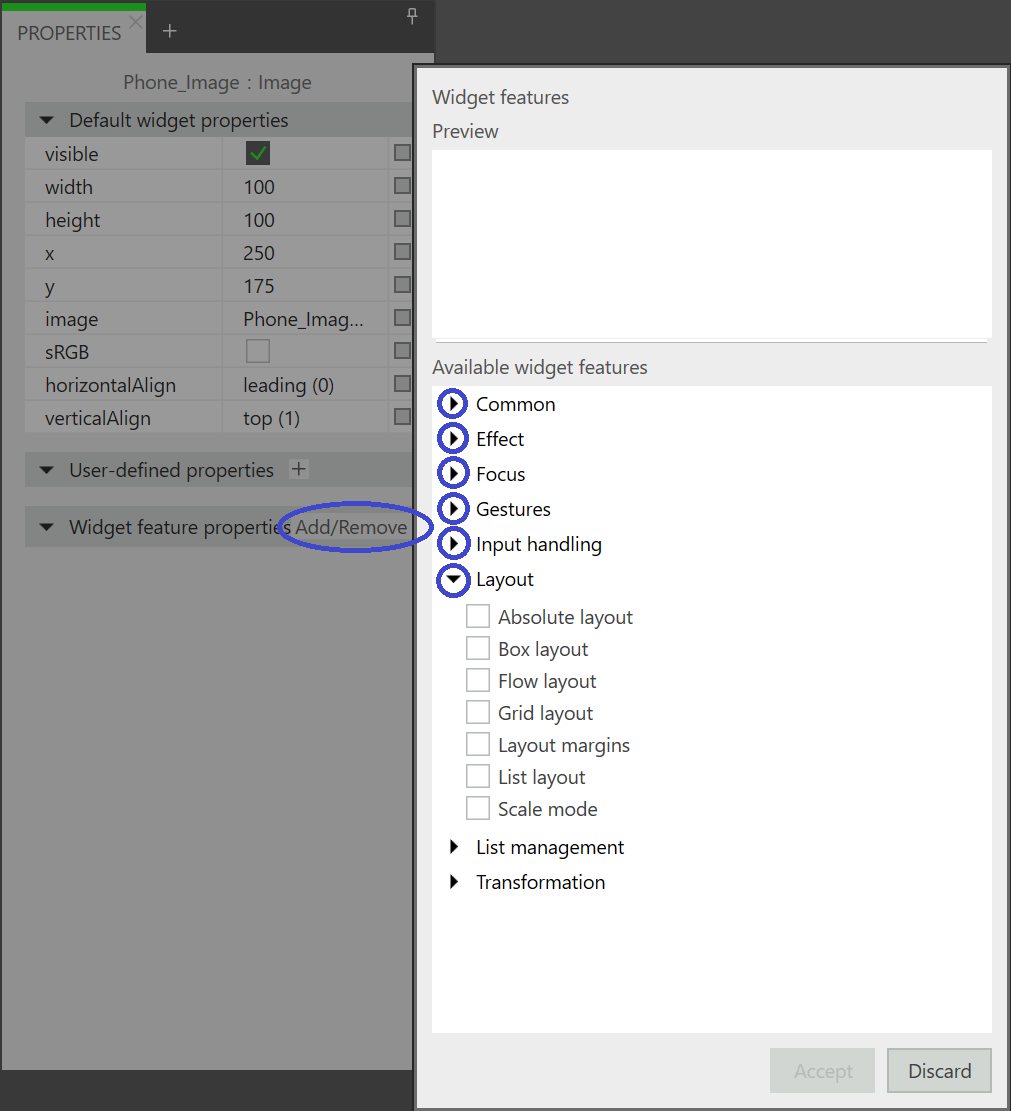
\includegraphics[scale=0.5]{figures/WidgetFeatureProperty.png}
  \captionof{figure}{Usability - Schwäche Widget Feature Properties}
  \label{fig:WidgetFeatureProperty}
\end{center}

\paragraph{Resultierende Benutzeranforderung}
Nutzer, die den Namen eine gewünschten Features wissen, müssen die Möglichkeit haben dieses Feature aus allen vorhanden herauszufiltern.

\paragraph{Mehrfachselektion}
Falls bei mehreren Objekten ein Property auf den gleichen Wert angepasst werden muss, ist es naheliegend für den Nutzer dies durch die zeitgleiche Selektion der betroffenen Elemente zu lösen.
Aktuell bietet EB Guide jedoch noch keine Unterstützung für Multiselektion, sind zwei Elemente ausgewählt sind diese lediglich gemeinsam mit der Maus bewegbar der View sieht wie in \cref{fig:Mehrfachselektion} zu sehen aus.

\begin{center}
  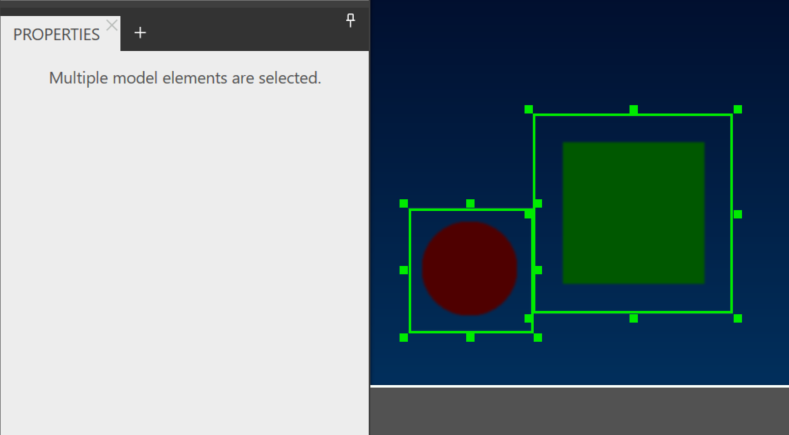
\includegraphics[scale=0.8]{figures/Mehrfachselektion.png}
  \captionof{figure}{Usability - Schwäche Mehrfachselektion}
  \label{fig:Mehrfachselektion}
\end{center}

\paragraph{Resultierende Benutzeranforderung}
Nutzer, die mehrere Objekte gleichzeitig selektiert haben, müssen die Möglichkeit haben all deren Properties nach ihren Wünschen zu verändern.

\section{Verbesserungen}
Da es Aufgrund der zeitlichen Einschränkungen dieser Arbeit nicht möglich ist alle aufgeführten Schwächen weiter zu analysieren wird im Folgenden erläutert auf welchen Grundlagen die Auswahl für die Verbesserungen getroffen wurde, welcher Gewinn für den Nutzer sich durch diese Verbesserungen versprochen wird und welches Design für die Verbesserungen angestrebt wird.

\subsection{Auswahlkriterien}
Ausgangspunkt für weiterführende Untersuchungen

\subsection{Gewinn für den Nutzer}
Effizienzsteigerung
intuitiver Bedienung


\subsection{Design der Verbesserungen}

\paragraph{Template Properties}

\begin{center}
  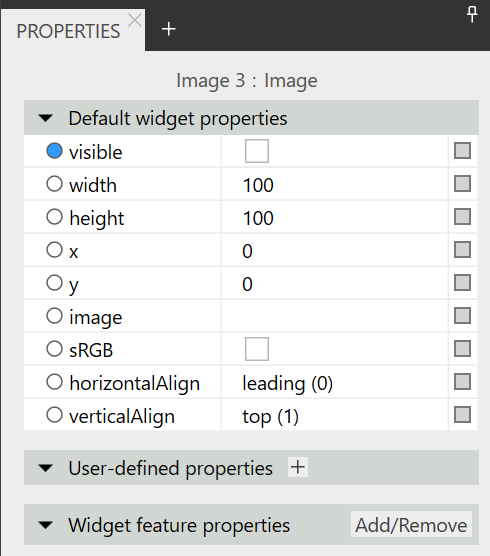
\includegraphics[scale=0.8]{figures/TemplateProperties_Adaption.png}
  \captionof{figure}{Verbesserung Template Properties}
  \label{fig:TemplateProperties_Adaption}
\end{center}


\paragraph{Widget Feature Properties}

\begin{center}
  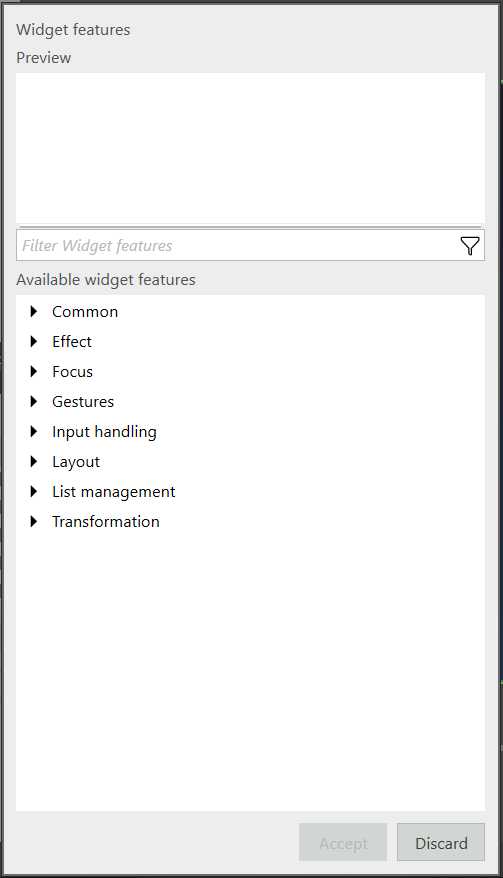
\includegraphics[scale=0.4]{figures/WidgetFeatureProperty_Adaption.png}
  \captionof{figure}{Verbesserung Feature Property Properties}
  \label{fig:FeatureProperty_Adaption}
\end{center}


\paragraph{Mehrfachselektion}

\begin{center}
  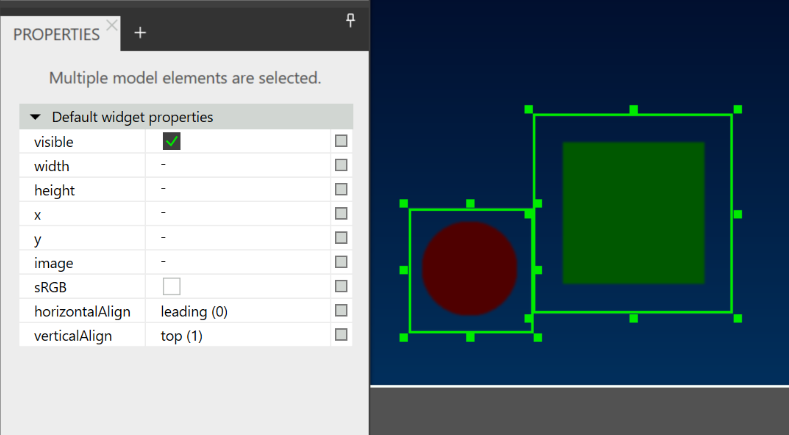
\includegraphics[scale=0.4]{figures/Mehrfachselektion_Adaption.png}
  \captionof{figure}{Verbesserung Mehrfachselektion}
  \label{fig:Mehrfachselektion_Adaption}
\end{center}

